\documentclass[BufferStockTheory]{subfiles}\providecommand{\econtexRoot}{}
\renewcommand{\econtexRoot}{..}

% WARNING: Different execution depending on whether
% 0. Being compiled as standalone document
% * Compile this file, then main, then this one again
% * Keep iterating until neither file changes
% 0. Being compiled as subfile of main document
% * Not clear what proper order is; might NOT matter

\onlyinsubfile{\externaldocument{BufferStockTheory}} % Get xrefs -- esp to appendix -- from main file; only works properly if main file has already been compiled; 

\begin{document}
\providecommand{\versn}{} % Version; like, web or pdf or journal submission
\ifthenelse{\boolean{ifWeb}}{  \renewcommand{\ushort}{\underline}\renewcommand{\versn}{Web} }{} % ushort does not work in tex4ht

\hfill{\tiny \jobname~\versn~\today, time:\DTMcurrenttime, source-commit: \input{.git-source-commit}, public-commit: \input{.git-public-commit}}

%%%\begin{verbatimwrite}{BufferStockTheory.title}  % Write title to .title file
%%%Theoretical Foundations of Buffer Stock Saving
%%%\end{verbatimwrite}

\title{Theoretical Foundations of \\ Buffer Stock Saving}

\author{Christopher D. Carroll\authNum}

\keywords{Precautionary saving, buffer stock saving, marginal propensity to consume, permanent income hypothesis}

\jelclass{D81, D91, E21}

\renewcommand{\forcedate}{September 28, 2020}
\date{\forcedate}

\maketitle %% Version finally sent back to QE, as MS 354
\hypertarget{abstract}{}
\begin{abstract}
This paper builds theoretical foundations for rigorous and intuitive understanding of `buffer stock' saving models, pairing each theoretical result with a quantitative exploration.  After describing conditions under which the consumption function converges, the paper shows that a `target' buffer stock exists only under conditions strictly stronger than those that guarantee convergence of the consumption and value functions.  It also shows that the average growth rate of consumption equals the average growth rate of permanent income (in a small open economy populated by buffer stock savers).  Together, the (provided) numerical tools and (proven) analytical results constitute a comprehensive toolkit for understanding buffer stock models.
\end{abstract}

% Various resources 
\hypertarget{links}{}
\begin{small}
\parbox{\textwidth}{
\begin{center}
\begin{tabbing}
\texttt{~Archive:~} \= \= \url{http://www.econ2.jhu.edu/people/ccarroll/BufferStockTheory.zip} \\  %
\texttt{~~~~~PDF:~} \> \> \url{http://llorracc.github.io/BufferStockTheory/BufferStockTheory.pdf} \\
\texttt{~~Slides:~} \> \> \url{http://llorracc.github.io/BufferStockTheory/BufferStockTheory-Slides.pdf} \\
\texttt{~~~~~Web:~} \> \> \url{http://llorracc.github.io/BufferStockTheory/BufferStockTheory/}    \\
\texttt{Appendix:~} \> \> \url{http://llorracc.github.io/BufferStockTheory/BufferStockTheory\#Appendices}    \\
%\texttt{~~bibtex:~} \> \> \url{http://llorracc.github.io/BufferStockTheory/BufferStockTheory.bib}  \\
\texttt{~~GitHub:~} \> \> \url{http://github.com/llorracc/BufferStockTheory} \\
\texttt{~~~~~~~~~~} \> \> \textit{(In GitHub repo, see \texttt{/Code} for tools for solving and simulating the model)} \\
\end{tabbing}
\end{center}
          
\href{https://econ-ark.org/materials/BufferStockTheory}{CLICK HERE} for an interactive \href{https://en.wikipedia.org/wiki/Project\_Jupyter\#Jupyter_Notebook}{Jupyter Notebook} that uses the \href{https://econ-ark/HARK}{Econ-ARK/HARK} toolkit to produce all of the paper's figures (warning: the notebook may take several minutes to launch).  Information about citing the toolkit can be found at \href{https://econ-ark.org/acknowledging/}{Acknowleding Econ-ARK}.
} % end parbox{\textwidth}
\end{small}

\begin{authorsinfo}
\name{Contact: \href{mailto:ccarroll@jhu.edu}{\texttt{ccarroll@jhu.edu}}, Department of Economics, 590 Wyman Hall, Johns Hopkins University, Baltimore, MD 21218, \url{http://econ.jhu.edu/people/ccarroll}, and National Bureau of Economic Research.}
\end{authorsinfo}

\thanks{All numerical results herein were produced using the \href{https://econ-ark/HARK}{Econ-ARK/HARK} toolkit, which can be cited per our references (\cite{carroll_et_al-proc-scipy-2018}); for reference to the toolkit itself see \href{https://econ-ark.org/acknowledging/}{Acknowleding Econ-ARK}.  Thanks to James Feigenbaum, Joseph Kaboski, Miles Kimball, Qingyin Ma, Misuzu Otsuka, Damiano Sandri, John Stachurski, Adam Szeidl, Metin Uyanik, Weifeng Wu, Xudong Zheng,
  and Jiaxiong Yao for comments on earlier versions of this paper, John Boyd for help
  in applying his weighted contraction mapping theorem, Ryoji
  Hiraguchi for extraordinary mathematical insight that improved the
  paper greatly, David Zervos for early guidance to the literature,
  and participants in a seminar at Johns Hopkins University and a
  presentation at the 2009 meetings of the Society of Economic
  Dynamics for their insights.}

\titlepagefinish


\newtheorem{defn}{Definition}
\newtheorem{theorem}{Theorem}

\hypertarget{Introduction}{}
\section{Introduction}

\label{sec:intro}

%%%Following the success of Modigliani and Brumberg's~\citeyearpar{modigliani&brumberg:lifecycle} Life Cycle model and Friedman's~\citeyearpar{friedmanATheory} Permanent Income Hypothesis, a vast literature in the 1960s and 1970s formalized the idea that household spending can be modeled as reflecting optimal intertemporal choice.  Bewley~\citeyearpar{bewleyPIH} and \cite{seIncFluct} capped this literature, paving the way for the ascendancy of dynamic stochastic optimizing models in economics.



In the presence of empirically realistic transitory and permanent shocks to income \textit{a la} \cite{friedmanATheory}, only one other ingredient is required to define a testable model of optimal consumption: A description of preferences.  Modelers usually assume geometric discounting of a constant relative risk aversion (CRRA) utility function, because, starting with Zeldes~\citeyearpar{zeldesStochastic}, a large literature has shown that models of this kind have quantitative predictions that can match microeconomic evidence reasonably well.

A companion theoretical literature has shown that standard numerical solution methods provide good approximations to limiting ``true'' mathematical solutions -- but only for models more complex than the simple case with just shocks and utility.  The extra complexity has been required because standard contraction mapping theorems (beginning with \cite{bellmanDynamicProgramming} and including those following Stokey et.~al.~\citeyearpar{slpMethods}) cannot be applied when the utility function is unbounded (like CRRA - see \hyperlink{DiffFromLit}{section \ref{subsec:Setup}}).\footnote{It is unclear whether newer methods such as those of \cite{mnUnique} could overcome this problem, or how difficult it would be to do so; but in any case this particular problem does not seem to have been tackled by those methods or any others.}

This paper's first technical contribution is to articulate the (surprisingly loose) conditions under which the simple problem (without convenient shortcuts like a consumption floor or liquidity constraints) defines a contraction mapping with a nondegenerate consumption function (the main requirement is a \hyperlink{FVAC}{`Finite Value of Autarky'} condition).  Another contribution is to specify the conditions under which the resulting consumption function implies there is a `target' wealth-to-permanent-income ratio (so the model exhibits `buffer stock' saving behavior.)  The key requirement for existence of a target is that the model's parameters satisfy a \hyperlink{GIC}{``Growth Impatience Condition''} (equation \eqref{eq:GIC}) that relates preferences and uncertainty to the predictable growth rate of income.

\hypertarget{KMP}{}

Even without a formal proof, target saving of this kind has been intuitively understood to underlie central numerical results from the heterogeneous agent macroeconomics literature; for example, the logic of target saving is central to the explanation by \cite{kmpHandbook} of the fact that, during the Great Recession, middle-class consumers cut their consumption more than the poor or the rich.  The theoretical logic articulated below explains this finding:  Learning that the future has become more uncertain does not change the urgent imperatives of the poor (their high $\uFunc^{\prime}(\cRat)$) because they have little room to maneuver.  Increased labor income uncertainty does not change the behavior of the rich because the increase in uncertainty does not threaten their consumption much.  Only people in the middle have both the motivation and the wiggle-room to reduce their discretionary spending.

Conveniently, elements required for the convergence proof turn out to provide analytical foundations for many other results that have become familiar from the numerical literature.  All theoretical conclusions are paired with numerically computed illustrations (using an open-source toolkit available from the \href{https://github.com/econ-ark/REMARK/blob/master/REMARKs/BufferStockTheory/BufferStockTheory.ipynb}{Econ-ARK} project).  All of the insights of this paper are instantiated in the toolkit, which algorithmically flags parametric choices under which a problem fails to define a contraction mapping, under which a target level of wealth does not exist, or under which the solution is otherwise degenerate.

Thus, the theoretical foundations provided here are valuable both because they provide intuition about the determinants of saving targets, and because they make it easier to develop reliable numerical solution methods (by providing tight restrictions that valid solutions must satisfy).

The paper proceeds in three parts.

The first part articulates the \hyperlink{Sufficient-Conditions}{conditions required} for the problem to define a unique nondegenerate limiting consumption function, and discusses the relation of the paper's model to models previously considered in the literature.  The required conditions are interestingly parallel to those required for the \hyperlink{Factors-Defined-And-Compared}{liquidity constrained perfect foresight model}; that parallel is explored and explained.  Next, the paper derives some limiting properties of the consumption function as cash approaches infinity and as it approaches its lower bound, and the theorem is proven explaining when the problem defines a contraction mapping.  Finally, a related class of commonly-used models (exemplified by Deaton~\citeyearpar{deatonLiqConstr}) is shown to constitute a particular limit of this paper's more general model.

The \hyperlink{AnalysisoftheConvergedConsumptionFunction}{next section} examines five key properties of the model. First, as \hyperlink{LimitsAsmtToInfty}{cash approaches infinity} the expected growth rate of consumption and the marginal propensity to consume (MPC) converge to their values in the perfect foresight case. Second, as \hyperlink{LimitsAsmtToZero}{cash approaches zero} the expected growth rate of consumption approaches infinity, and the MPC approaches a simple analytical limit.  Third, if the consumer is `growth impatient,' a \hyperlink{onetarget}{unique target cash-to-permanent-income ratio} will exist.  Fourth, at the target cash ratio, the \hyperlink{cGroLTpGro}{expected growth rate of consumption} is slightly less than the expected growth rate of permanent noncapital income.  Finally, the expected growth rate of consumption \hyperlink{dcgdxneg}{is declining in the level of cash}. The first four propositions are proven under general assumptions about parameter values; the last is shown to hold if there are no transitory shocks, but may fail in extreme cases if there are both transitory and permanent shocks.

Szeidl~\citeyearpar{szeidlInvariant} has shown that such an economy will be characterized by stable invariant distributions for the consumption ratio, the wealth ratio, and other variables.\footnote{Szeidl's proof supplants the analysis in an earlier draft of this paper, which conjectured that such a result held and provided supportive simulation evidence.}  Using Szeidl's result, the final section discusses conditions under which, even with a fixed aggregate interest rate that differs from the time preference rate, an economy populated by buffer stock consumers converges to a balanced growth equilibrium in which the growth rate of consumption tends toward the (exogenous) growth rate of permanent income.

\hypertarget{The-Problem}{}
\section{The Problem}

\subsection{Setup}
\label{subsec:Setup}

The consumer solves an optimization problem from period
$t$ until the end of life at $T$ defined by the objective
\begin{verbatimwrite}{\EqDir/supfn.tex}
\begin{align}
  \label{eq:supfn}
  \max~ \Ex_{t}\left[\sum_{n=0}^{T-t} \DiscFac^{n} \uFunc(\cLevBF_{t+n})\right]
\end{align}
\end{verbatimwrite}
  \begin{align*}%    \label{eq:supfn}
    \max~ \Ex_{t}\left[\sum_{n=0}^{T-t} \DiscFac^{n} \uFunc(\cLevBF_{t+n})\right]
  \end{align*}

where
\begin{align}
  \uFunc(\bullet)=\bullet^{1-\CRRA}/(1-\CRRA) \label{eq:crrautil}
\end{align}
 is a constant relative risk aversion utility function with $\CRRA > 1$.\footnote{The main
  results also hold for logarithmic utility which is the limit as
  $\CRRA \rightarrow 1$ but incorporating the logarithmic special case
  in the proofs is cumbersome and therefore
  omitted.}$^{,}$\footnote{We will define the infinite horizon
  solution as the limit of the finite horizon problem as the horizon
  $T-t$ approaches infinity.}  The consumer's initial condition is
defined by market resources $\mLevBF_{t}$ (which \cite{deatonLiqConstr}
called `cash-on-hand') and permanent noncapital income $\pLevBF_{t}$.

In the usual treatment, a dynamic budget constraint (DBC) simultaneously incorporates
all of the elements that determine next period's $\mLevBF$ given this
period's choices; but for the detailed analysis here, it will be useful to
disarticulate the steps so that individual ingredients can be separately examined:

\begin{verbatimwrite}{\EqDir/DBCparts.tex}
\begin{align}
\aLevBF_{t}    & = \mLevBF_{t}-\cLevBF_{t}  \label{eq:DBCparts} \\
\bLevBF_{t+1}    & = \aLevBF_{t} \Rfree \notag \\
\pLevBF_{t+1}  & = \pLevBF_{t} \underbrace{\PGro\pShk_{t+1}}_{\equiv \PGro_{t+1}}  \notag \\
\mLevBF_{t+1}  & =  \bLevBF_{t+1} +\pLevBF_{t+1}\tShkAll_{t+1},  \notag
\end{align}
\end{verbatimwrite}

  \begin{equation}\begin{gathered}\begin{aligned}
    \aLevBF_{t}    & = \mLevBF_{t}-\cLevBF_{t}  \label{eq:DBCparts} \\
    \bLevBF_{t+1}    & = \aLevBF_{t} \Rfree \notag \\
    \pLevBF_{t+1}  & = \pLevBF_{t} \underbrace{\PGro\pShk_{t+1}}_{\equiv \PGro_{t+1}}  \notag \\
    \mLevBF_{t+1}  & =  \bLevBF_{t+1} +\pLevBF_{t+1}\tShkAll_{t+1},  \notag
  \end{aligned}\end{gathered}\end{equation}
 where $\aLevBF_{t}$ indicates the consumer's assets at the end of period $t$, which grow by a fixed interest factor $\Rfree =(1+\rfree)$ between periods,\footnote{See \cite{mstCapIncFluct} for interesting new work that considers the case where capital returns are stochastic and liquidity constraints exist.  \cite{benhabibWealth} examines implications of capital income risk for the distribution of wealth.}  so that $\bLevBF_{t+1}$ is the consumer's financial (`bank') balances before next period's consumption choice;\footnote{Allowing a stochastic interest factor is straightforward but adds little insight.  The effects are more interesting for analysis of the invariant distribution (\cite{szeidlInvariant}).} $\mLevBF_{t+1}$ (`market resources' or `money') is the sum of financial wealth $\bLevBF_{t+1}$ and noncapital income $\pLevBF_{t+1}\tShkAll_{t+1}$ (permanent noncapital income $\pLevBF_{t+1}$ multiplied by a mean-one iid transitory income shock factor $\tShkAll_{t+1}$; future transitory shocks are assumed to satisfy $\Ex_{t}[{\tShkAll}_{t+n}]=1~\forall~n\geq 1$). Permanent noncapital income in period $t+1$ is equal to its previous value, multiplied by a growth factor $\PGro$, modified by a mean-one iid shock $\pShk_{t+1}$, $\Ex_{t}[{\pShk}_{t+n}]=1~\forall~n \geq 1$ satisfying $\pShk \in [\ushort{\pShk},\bar{\pShk}]$ for $0 < \ushort{\pShk} \leq 1 \leq \bar{\pShk} < \infty$ where \tracingassigns=1\tracingmacros=1
$\ushort{\pShk}=\bar{\pShk}=1$ is the degenerate case with no permanent shocks.\footnote{It is useful to emphasize that permanent noncapital income as defined here differs from what Deaton~\citeyearpar{deatonUnderstandingC} calls permanent income (which is often adopted in the macro literature).  Deaton defines permanent income as the amount that a perfect foresight consumer could spend while leaving total (human and nonhuman) wealth constant.  Relatedly, we refer to $\mLevBF_{t}$ as `cash-on-hand' or `market resources' rather than as wealth to avoid any confusion for readers accustomed to thinking of the discounted value of future noncapital income as a part of wealth.  The `market resources' terminology is motivated by the model's assumption that human wealth cannot be capitalized, an implication of anti-slavery laws.}$^{,}$\footnote{Hereafter for brevity we occasionally drop time subscripts, e.g.\ $\Ex[\pShk^{-\CRRA}]$ signifies $\Ex_{t}[\pShk_{t+1}^{-\CRRA}]$.}


In future periods $t+n ~\forall~ n \geq 1$ there is a small probability $\pZero$ that income will
be zero (a `zero-income event'),
\begin{verbatimwrite}{\EqDir/tShkDef}
\begin{equation}
\tShkAll _{t+n}=
\begin{cases}
 0\phantom{_{t+1}/\pNotZero} & \text{with probability $\pZero>0$} \\
 \tShkEmp_{t+n}/\pNotZero      & \text{with probability $\pNotZero  $} % \equiv (1-\pZero) 
\end{cases} \label{eq:tShkDef}
\end{equation}
\end{verbatimwrite}
\begin{equation}
\tShkAll _{t+n}=
\begin{cases}
 0\phantom{_{t+1}/\pNotZero} & \text{with probability $\pZero>0$} \\
 \tShkEmp_{t+n}/\pNotZero      & \text{with probability $\pNotZero  $} % \equiv (1-\pZero)
\end{cases} \label{eq:tShkDef}
\end{equation}

where $\tShkEmp_{t+n}$ is an iid mean-one random variable
($\Ex_{t}[{\tShkEmp}_{t+n}]=1~\forall~n>0$)
that has a distribution
satisfying $\tShkEmp \in \lbrack \ushort{\tShkEmp},\bar{\tShkEmp}\rbrack$
where $0<\ushort{\tShkEmp} \leq 1 \leq \bar{\tShkEmp}<\infty$
(degenerately $\ushort{\tShkEmp}=\bar{\tShkEmp}=1$). (See \cite{rabaultBorrowing} and \cite{lsIncFluct} for analyses of cases where the shock processes have unbounded support).  Call the cumulative
distribution functions $\CDF_{\pShk}$ and $\CDF_{\tShkEmp}$ (and $\CDF_{\tShkAll}$
is derived trivially from \eqref{eq:tShkDef} and $\CDF_{\tShkEmp}$).
Permanent income and cash start out strictly positive, $\{\pLevBF_{t},\mLevBF_{t}\} \in
(0,\infty)$, and as usual the consumer cannot die in
debt, so
\begin{align}
  \cLevBF_{T} & \leq  \mLevBF_{T} \label{eq:NoDebtAtDeath}.
\end{align}

\hypertarget{PDV}{}
The model looks more special than it is.  In particular, the
assumption of a positive probability of zero-income events may seem
objectionable.  However, it is easy to show that a model with a
nonzero minimum value of $\tShkAll$ (motivated, for example, by the
existence of unemployment insurance) can be redefined by capitalizing
the present discounted value of minimum income into current market assets,\footnote{So long
  as this PDV is a finite number and unemployment benefits are
  proportional to $\pLevBF_{t}$; see the discussion in
  section~\ref{sec:discussConvergence}.}  analytically transforming
that model back into the model analyzed here.  Also, the assumption of
a positive point mass (as opposed to positive density) for the worst
realization of the transitory shock is inessential, but simplifies the proofs and is a powerful aid to intuition.\footnote{No key results would change if the unemployment state were persistent but mean-reverting, instead of IID.}

\begin{comment}
Combining the transition equations, the recursive nature of
the problem allows us to rewrite it more compactly in Bellman equation form,
\begin{align*}
\VFunc_{t}(\mLevBF_{t},\pLevBF_{t})  & = \max_{\cLevBF_{t}}~\left\{\uFunc(\cLevBF_{t})+\DiscFac \Ex_{t}\left[ \VFunc_{t+1}((\mLevBF_{t}-\cLevBF_{t})\Rfree+ \pLevBF_{t+1}\tShkAll_{t+1},\pLevBF_{t} \PGro  \pShk_{t+1})\right]\right\}
.
\end{align*}
\end{comment}

\hypertarget{DiffWithLit}{} This model differs from Bewley's~\citeyearpar{bewleyPIH} classic formulation in several ways. The CRRA utility function does not satisfy Bewley's assumption that $\uFunc(0)$ is well defined, or that $\uP(0)$ is well defined and finite, so neither the value function nor the marginal value function will be bounded.  It differs from Schectman and Escudero~\citeyearpar{seIncFluct} in that they impose liquidity constraints and positive minimum income.  It differs from both of these in that it permits permanent growth in income, and also permanent shocks to income, which a large empirical literature finds are quantitatively important in micro data\footnote{MaCurdy~\citeyearpar{macurdyTimeseries}; Abowd and Card~\citeyearpar{acCovariance}; Carroll and Samwick~\citeyearpar{csNature}; Jappelli and Pistaferri~\citeyearpar{jpCins}; Storesletten, Telmer, and Yaron~\citeyearpar{styConsumption}; \cite{blpRisk}} and which since~\cite{friedmanATheory} have been understood to be far more consequential for household welfare than are transitory fluctuations.  It differs from Deaton~\citeyearpar{deatonLiqConstr} because liquidity constraints are absent; there are separate transitory and permanent shocks ({\it a la} \cite{muthOptimal}); and the transitory shocks here can occasionally cause income to reach zero.\footnote{Below it will become clear that the Deaton model is a particular limit of this paper's model.}  Finally, it differs from models found in Stokey et.\ al.~\citeyearpar{slpMethods} because neither liquidity constraints nor bounds on utility or marginal utility are imposed.\footnote{Similar restrictions to those in the cited literature are made in the well known papers by Scheinkman and Weiss~\citeyearpar{scheinkman&weiss:borrowing} and Clarida~\citeyearpar{claridaErgodic}.  See \cite{tocheUrisk} for an elegant analysis of a related but simpler continuous-time model.}  \cite{asHomogeneous} relaxed the bounds on the return function, but they address only the deterministic case.

The incorporation of permanent shocks rules out application of the tools of \cite{mnUnique}, who followed and corrected an error in the fundamental work on the local contraction mapping method developed in \cite{rrExistence}.  \cite{mvExistence} provides a correction to \cite{rrExistence}, and provides conditions that are easier to verify than those of \cite{rrExistence} in many applications, but again only addresses the deterministic case.  

\hypertarget{The-Problem-Can-Be-Rewritten-in-Ratio-Form}{}
\subsection{The Problem Can Be Rewritten in Ratio Form}

\label{subsec:ratio}

We establish a bit more notation by reviewing the standard result that in problems of this class (CRRA utility, permanent shocks) the number of relevant state variables can be reduced from two ($\mLevBF$ and $\pLevBF$) to one $(\mRat = \mLevBF/\pLevBF)$.  Defining nonbold variables as the boldface counterpart normalized by $\pLevBF_{t}$ (as with $\mRat$ just above), assume that value in the last period of life is $\uFunc(\mLevBF_{T})$, and consider the problem in the second-to-last period,
\begin{align}
\vLevBF_{T-1}(\mLevBF_{T-1},\pLevBF_{T-1})  & = 
\max_{\cLevBF_{T-1}}~ \uFunc(\cLevBF_{T-1}) +\DiscFac \Ex_{T-1} [ \uFunc(\mLevBF_{T})]
\notag \\
 & =  \max_{\cRat_{T-1}}~
\uFunc(\pLevBF_{T-1}\cRat_{T-1}) + \DiscFac  \Ex_{T-1} [\uFunc(\pLevBF_{T}{\mRat}
_{T})]  \notag \\
 & = \pLevBF_{T-1}^{1-\CRRA}
\left\{\max_{\cRat_{T-1}}~ \uFunc(c_{T-1}) + \DiscFac \Ex_{T-1} [ \uFunc( {\PGro}_{T}
{\mRat}_{T}) ] \right\}  . \label{eq:vBold}
\end{align}
where the last line follows because for the CRRA utility function in \eqref{eq:crrautil}, $\uFunc(xy) =
x^{1-\CRRA}\uFunc(y)$.

\hypertarget{The-Related-Problem}{}
Now, in a one-time deviation from the notational convention established in the last paragraph, define nonbold `normalized value' not as $\vLevBF_{t}/\pLevBF_{t}$ but as $\vFunc_{t} = \vLevBF_{t}/\pLevBF_{t}^{1-\CRRA}$, because this allows us to use the related problem 
%%\begin{verbatimwrite}{\EqDir/veqn.tex} % Weirdly, if \label{eq:veqn} is in verbatimwritten file, reference is not correctly constructed, so comment out verbatimrwite here
\begin{align}
\vFunc_{t}(\mRat_{t})  & = \max_{\{\cFunc\}_{t}^{T}}~  \uFunc(\cFunc_{t}) +\DiscFac \Ex_{t}[\PGro_{t+1}^{1-\CRRA}\vFunc_{t+1}({\mRat}_{t+1})] \notag \\
& \mbox{s.t.}  \label{eq:veqn} 
 \\ {\aRat}_{t}  & = \mRat_{t}-c_{t}  \notag
 \\ {\bRat}_{t+1}  & = (\Rfree/\PGro_{t+1})\aRat_{t}  ~ = ~ \Rnorm_{t+1}\aRat_{t}  \notag
\\ \mRat_{t+1}  & = \bRat_{t+1}+\tShkAll_{t+1}  \notag %
\end{align}
%%\end{verbatimwrite}\begin{eqnarray}
\vFunc_{t}(\mRat_{t}) & = & \max_{\{\cFunc\}_{t}^{T}}~  \util(\cFunc_{t}) +\DiscFac \Ex_{t}[\PGro_{t+1}^{1-\CRRA}\vFunc_{t+1}({\mRat}_{t+1})] \notag \\
& \mbox{s.t.} &  \label{eq:veqn} \notag
 \\ {\aRat}_{t} & = & \mRat_{t}-c_{t}  \notag
 \\ {\bRat}_{t+1} & = & (\Rfree/\PGro_{t+1})\aRat_{t}  ~ = ~ \Rnorm_{t+1}\aRat_{t}  \notag
\\ \mRat_{t+1} & = & \bRat_{t+1}+\tShkAll_{t+1}  \notag %
\end{eqnarray}

where $\Rnorm_{t+1}\equiv (\Rfree/\PGro_{t+1})$ is a `growth-normalized' return factor, and the problem's first order condition is
\begin{align}
c_{t}^{-\CRRA}  & = \Rfree \DiscFac \Ex_{t}[ {\PGro}_{t+1}^{-\CRRA} {\cRat}
_{t+1}^{-\CRRA}].  \label{eq:scaledeuler}
\end{align}

Since $\vFunc_{T}(\mRat_{T}) = \uFunc(\mRat_{T})$, defining $\vFunc_{T-1}(\mRat_{T-1})$ from \eqref{eq:veqn} for $t=T-1$, \eqref{eq:vBold} reduces to
\begin{align*}
\vLevBF_{T-1}(\mLevBF_{T-1},\pLevBF_{T-1})  & = \pLevBF_{T-1}^{1-\CRRA} \vFunc_{T-1}(\underbrace{\mLevBF_{T-1}/\pLevBF_{T-1}}_{=\mRat_{T-1}}).
\end{align*}

This logic induces to all earlier periods, so that if we solve the
normalized one-state-variable problem specified in \eqref{eq:veqn} we
will have solutions to the original problem for any $t<T$
from:
\begin{align*}
   \vLevBF_{t}(\mLevBF_{t},\pLevBF_{t})  & = \pLevBF_{t}^{1-\CRRA}\vFunc_{t}(\mRat_{t}),
\\ \cLevBF_{t}(\mLevBF_{t},\pLevBF_{t})  & = \pLevBF_{t}\cFunc_{t}(\mRat_{t}).
\end{align*}

\hypertarget{Definition-of-a-Nondegenerate-Solution}{}
\subsection{Definition of a Nondegenerate Solution}

We say that this problem has a nondegenerate solution if, as the number of remaining periods of life gets arbitrarily large, it
defines a unique limiting consumption function whose optimal
$\cRat$ satisfies
\begin{align}
  0 & < \cRat <  \infty 
\end{align}
for every $0 < \mRat < \infty.$ (`Degenerate' limits will be cases
where the limiting consumption function is either $\cFunc(\mRat)=0$ or $\cFunc(\mRat)=\infty$.)

\hypertarget{Perfect-Foresight-Benchmarks}{}
\subsection{Perfect Foresight Benchmarks}

Articulating the familiar analytical solution to the perfect foresight specialization of the model, obtained by setting $\pZero=0$ and $\ushort{\tShkEmp}=\bar{\tShkEmp}=\ushort{\pShk}=\bar{\pShk}=1$, allows us to define some remaining notation and terminology, and to define a convenient reference point.

\hypertarget{Human-Wealth}{}
\subsubsection{Human Wealth}
The dynamic budget constraint, strictly positive marginal utility, and the can't-die-in-debt condition \eqref{eq:NoDebtAtDeath} imply an exactly-holding intertemporal budget constraint (IBC)
\begin{align}
  \text{PDV}_{t}(\cLevBF)  & = \overbrace{\mLevBF_{t}-\pLevBF_{t}}^{\bLevBF_{t}}+\overbrace{\text{PDV}_{t}(\pLevBF)}^{\hLevBF_{t}}, \label{eq:IBCFinite}
\end{align}
where $\bLevBF$ is nonhuman wealth and $\hLevBF_{t}$ is `human wealth,' and with a constant $\Rnorm \equiv \Rfree/\PGro$,
\begin{align}
  \hLevBF_{t}  & = \pLevBF_{t}+\Rnorm^{-1} \pLevBF_{t} + \Rnorm^{-2} \pLevBF_{t} + ... + \Rnorm^{t-T} \pLevBF_{t} \notag
\\  & = \underbrace{\left(\frac{1-\Rnorm^{-(T-t+1)}}{1-\Rnorm^{-1}}\right)}_{\equiv \hRat_{t}}\pLevBF_{t} \label{eq:HDef}.
\end{align}
Equation \eqref{eq:HDef} makes plain that in order for $\hRat \equiv \lim_{n \rightarrow
  \infty} \hRat_{T-n}$ to be finite, we must
impose the Finite Human Wealth Condition (`FHWC') \hypertarget{FHWC}{}
\begin{align}
  \underbrace{\PGro/\Rfree}_{\equiv \Rnorm^{-1}}  & < 1 \label{eq:FHWC}.
\end{align}
Intuitively, for human wealth to be finite, the growth rate of (noncapital) income must be smaller than
the interest rate at which that income is being discounted.

\hypertarget{Unconstrained-Solution}{}
\subsubsection{Unconstrained Solution} \label{subsec:PFUncon}

\hypertarget{APF}{}
\hypertarget{AIC}{}
The consumption Euler equation holds in every period; with $\uP(\cLevBF)=\cLevBF^{-\CRRA}$, this says\hypertarget{Pat}{}
\begin{align}
%%  \cLevBF_{t}^{-\CRRA}  & = \Rfree\DiscFac \cLevBF_{t+1}^{-\CRRA} \\ \notag
 \cLevBF_{t+1}/\cLevBF_{t}  & = (\Rfree\DiscFac)^{1/\CRRA} \equiv \Pat   \label{eq:Pat}
\end{align}
where the Old English letter `thorn' represents what we will call the
`absolute patience factor' $(\Rfree
\DiscFac)^{1/\CRRA}$.\footnote{Impatience conditions of one kind or
  another have figured in intertemporal optimization problems since
  such problems were first formalized in economics, most notably by \cite{ramseySave}.
  Discussion of these issues was prominent in the literature of the
  1960s and 1970s, and no brief citations here could do justice to the literature on the topic, so I refrain from the attempt.}  The sense in which $\Pat$ captures
patience is that if the `absolute impatience condition' (\AIC) holds,
\begin{align}
  \label{eq:AIC}
  \Pat  & < 1,
\end{align}
the consumer will choose to spend an amount too large to sustain indefinitely (the
level of consumption must fall over time).  We call such a consumer `absolutely impatient' (this is the key condition in \cite{bewleyPIH}).

We next define a `return patience factor' that relates absolute patience to the return factor:
\begin{align}
 \PatR  & \equiv  {\Pat}/\Rfree \label{eq:PatR}
\end{align}
and note that since consumption is growing by $\Pat$ but discounted by $\Rfree$:
\begin{align}
  \text{PDV}_{t}(\cLevBF)  & = \left(1+\PatR+\PatR^{2}+...+ \PatR^{T-t}\right)\cLevBF_{t} \notag
\\  & = \left(\frac{1-\PatR^{T-t+1}}{1-\PatR}\right)\cLevBF_{t}
\end{align}
from which the IBC \eqref{eq:IBCFinite} implies
\begin{align}
  \cLevBF_{t}  & = \overbrace{\left(\frac{1-\PatR}{1-\PatR^{T-t+1}}\right)}^{\equiv \MinMPC_{t}}
(\bLevBF_{t}+\hLevBF_{t})   \label{eq:WDef}
\end{align}
which defines a normalized finite-horizon perfect foresight consumption function
\begin{align}
  \bar{\cFunc}_{T-n}(\mRat_{T-n})  & = (\overbrace{\mRat_{T-n}-1}^{=\bRat_{T-n}}+\hRat_{T-n})\MinMPC_{T-n}
\end{align}
where $\MinMPC_{t}$ is the marginal propensity to consume (MPC) because it answers the
question `if the consumer had an extra unit of wealth, how much more would he spend.' \hypertarget{RIC}{}
(The overbar on $\cFunc$ reflects the fact that this will be an upper bound as we modify the problem to incorporate constraints and uncertainty; analogously, the underbar for $\MPC$ indicates that it is a lower bound).
Equation \eqref{eq:WDef} makes plain that for the limiting
MPC to be strictly positive as $n=T-t$ goes to infinity we must impose the Return Impatience Condition:
condition 
\begin{align}
\PatR  & < 1   \label{eq:RIC},
\end{align}
so that
\begin{align}
   0 <  \MinMPC  & \equiv   1-\PatR = \lim_{n \rightarrow \infty} \MinMPC_{T-n} \label{eq:MinMPCDef}
.
\end{align}

Equation \eqref{eq:RIC} thus imposes a second kind of `impatience:' The consumer cannot be so pathologically patient as to wish, in the limit as the horizon approaches infinity, to spend nothing today out of an increase in current wealth; that is, the condition rules out the degenerate limiting solution $\bar{\cFunc}(\mRat)=0$.  Because the return patience factor $\PatR$ is the absolute patience factor divided by the return, we call equation \eqref{eq:RIC} the `return impatience condition' or \RIC; we will say that a consumer who satisfies the condition is `return impatient.'

Given that the \RIC~holds, and defining limiting objects by the absence of a time subscript (e.g., $\bar{\cFunc}(\mRat)=\lim_{n \uparrow \infty} \bar{\cFunc}_{T-n}(\mRat)$), the limiting consumption function will be
\begin{align}\label{eq:cFuncPFUnc}
  \bar{\cFunc}(\mRat)  & = (\mRat+\hRat-1)\MinMPC, 
\end{align}
and we now see that in order to rule out the degenerate limiting
solution $\bar{\cFunc}(\mRat) = \infty$ we need $\hRat$ to be finite so we
must impose the finite human wealth condition \eqref{eq:FHWC}.

\hypertarget{ValuePFAnalytical}{}
A final useful point is that since the perfect foresight
growth factor for consumption is $\Pat$, again using $\uFunc(xy) =
x^{1-\CRRA}\uFunc(y)$, yields an analytical expression for value:  
\begin{align}
  \vRat_{t}  & = \uFunc(\cRat_{t})+\DiscFac \uFunc(\cRat_{t}\Pat)+\DiscFac^{2} \uFunc(\cRat_{t} \Pat^{2})+... \label{eq:ValuePFAnalytical}
\\  & = \uFunc(\cRat_{t})\left(1+\DiscFac \Pat^{1-\CRRA}+(\DiscFac \Pat^{1-\CRRA})^{2}+...\right) \notag 
\\  & = \uFunc(\cRat_{t})\left(\frac{1-(\DiscFac \Pat^{1-\CRRA})^{T-t+1}}{1-\DiscFac \Pat^{1-\CRRA}}\right) \notag
\end{align}
which asymptotes to a finite number as $n=T-t$ approaches $+\infty$ if $\DiscFac \Pat^{1-\CRRA} < 1$ (related to a condition in \cite{asHomogeneous}); with a bit of algebra, this requirement can be shown to be equivalent to the \RIC.\footnote{
\begin{align*}
   \DiscFac ((\Rfree \DiscFac)^{1/\CRRA})^{1-\CRRA}  & < 1
%%\\ \DiscFac (\Rfree\DiscFac)^{(1-\CRRA)/\CRRA}  & < 1
\\ \DiscFac (\Rfree\DiscFac)^{1/\CRRA}/\Rfree\DiscFac  & < 1
\\ (\Rfree \DiscFac)^{1/\CRRA} /\Rfree  & < 1
\end{align*}.
}  Thus, the same conditions that guarantee a nondegenerate limiting consumption function also guarantee a nondegenerate limiting value function (which will \textit{not} be true in the version of the model that incorporates uncertainty).


\hypertarget{Constrained-Solution}{}
\subsubsection{Constrained Solution}

If a liquidity constraint requiring $\bRat \geq 0$ is ever to be relevant, it must be
relevant at the lowest possible level of market resources,
$\mRat_{t}=1$, which obtains for a consumer who enters period $t$ with
$\bRat_{t}=0$.  The constraint is `relevant' if
it prevents the choice that would otherwise be optimal; at
$\mRat_{t}=1$ the constraint is relevant if the marginal utility from spending all of today's
resources $c_{t}=m_{t}=1$, exceeds the marginal utility from
doing the same thing next period, $\cRat_{t+1}=1$; that is, if such
choices would violate the Euler equation \eqref{eq:scaledeuler}:
\begin{align}
    1^{-\CRRA}  & > \Rfree \DiscFac (\PGro)^{-\CRRA}1^{-\CRRA}  \label{eq:LiqConstrBinds}.
\end{align}

\hypertarget{PFGPF}{}
\hypertarget{PFGIC}{}
By analogy to the return patience factor, we therefore define a `perfect
foresight growth patience factor' as
\begin{align}
  \PatPGro  & = {\Pat}/\PGro,  \label{eq:PFGPF}
\end{align}
and define a `perfect foresight growth impatience condition' (\PFGIC)
\begin{align}
  \label{eq:PFGIC}
  \PatPGro &  < 1
\end{align}
which is equivalent to \eqref{eq:LiqConstrBinds} (exponentiate both
sides by $1/\CRRA$).

If the \RIC~and the \FHWC~hold, appendix \ref{sec:ApndxLiqConstr} shows
that, for some $0 < \mRat_{\#} < 1$, an unconstrained consumer behaving according to
\eqref{eq:cFuncPFUnc} would choose $\cRat < \mRat$ for all $\mRat >
\mRat_{\#}$.  The solution to the
constrained consumer's problem in this case is simple: For any $\mRat
\geq \mRat_{\#}$ the constraint does not bind (and will never bind in
the future) and so the constrained consumption function is identical
to the unconstrained one.  If the consumer were somehow\footnote{``Somehow'' because $\mRat<1$ could only be
obtained by entering the period with $\bRat < 0$ which the constraint
forbids.}
to arrive at an $\mRat < \mRat_{\#} < 1$ the constraint would bind and
the consumer would have to consume $\cRat=\mRat$.  We use the $\circ$ accent to designate the limiting
constrained consumption function:
\begin{equation}
\mathring{\cFunc}(\mRat)=
\begin{cases}
 \mRat & \text{if $\mRat < \mRat_{\#}$} \\
 \bar{\cFunc}(\mRat)  & \text{if $\mRat \geq \mRat_{\#}$.}
\end{cases}
\end{equation}

More useful is the case where the perfect foresight growth and return impatience conditions both hold.  In this case appendix \ref{sec:ApndxLiqConstr} shows that the limiting constrained consumption function is piecewise linear, with $\mathring{\cFunc}(\mRat)=\mRat$ up to a first `kink point' at $\mRat_{\#}^{1}>1$, and with discrete declines in the MPC at successively increasing kink points $\{\mRat_{\#}^{1},\mRat_{\#}^{2},...\}$.  As $\mRat \uparrow \infty$ the constrained consumption function $\mathring{\cFunc}(\mRat)$ becomes arbitrarily close to the unconstrained $\bar{\cFunc}(\mRat)$, and the marginal propensity to consume function $\mathring{\MPCFunc}(\mRat) \equiv \mathring{\cFunc}^{\prime}(\mRat)$ limits to $\MinMPC$.  Similarly, the value function $\mathring{\vFunc}(\mRat)$ is nondegenerate and limits into the value function of the unconstrained consumer.  Surprisingly, this logic holds even when the finite human wealth condition fails (denoted \cncl{\FHWC}).  A solution exists because the constraint prevents the consumer from borrowing against infinite human wealth to finance infinite current consumption.  Under these circumstances, the consumer who starts with any amount of resources $\bRat_{t} > 1$ will, over time, run those resources down so that by some finite number of periods $n$ in the future the consumer will reach $\bRat_{t+n} = 0$, and thereafter will set $\cRat = \mRat = 1$ for eternity, a policy that will (using \eqref{eq:ValuePFAnalytical}) yield value of \hypertarget{PFFVAC}{}
\begin{align}
  \vLevBF_{t+n}  & = \uFunc(\pLevBF_{t+n})\left(1+\DiscFac
    \PGro^{1-\CRRA}+(\DiscFac \PGro^{1-\CRRA})^{2}+...\right) \notag
  \\  & = \PGro^{n(1-\CRRA)} \uFunc(\pLevBF_{t})\left(\frac{1-(\DiscFac
      \PGro^{1-\CRRA})^{T-(t+n)+1}}{1-\DiscFac \PGro^{1-\CRRA}}\right),
  \notag
\end{align}
which will be finite whenever 
\begin{align}
   \overbrace{\DiscFac \PGro^{1-\CRRA} }^{\equiv \DiscAlt}  & < 1 \label{eq:PFFVAC}
\\ \DiscFac \Rfree \PGro^{-\CRRA}  & < \Rfree/\PGro \nonumber
\\ \PatPGro  & < (\Rfree/\PGro)^{1/\CRRA} \nonumber
\end{align}
which we call the Perfect Foresight Finite Value of Autarky Condition, \PFFVAC, because it guarantees that a consumer who always spends all his permanent income will have finite value (the consumer has `finite autarky value').  Note that the version of the \PFFVAC~in \eqref{eq:PFFVAC} implies the \PFGIC~$\PatPGro < 1$ whenever \cncl{\FHWC} ($\Rfree < \PGro$) holds.  So, if \cncl{\FHWC}, value for any finite $\mRat$ will be the sum of two finite numbers: The component due to the unconstrained consumption choice made over the finite horizon leading up to $\bRat_{t+n} = 0$, and the finite component due to the value of consuming all income thereafter.  The consumer's value function is therefore nondegenerate.

The most peculiar possibility occurs when the \RIC~fails.  The appendix shows that under these circumstances the \FHWC~must also fail, and the constrained consumption function is nondegenerate.  (See Figure~\ref{fig:PFGICHoldsFHWCFailsRICFails} for a numerical example).  While it is true that $\lim_{m \uparrow \infty}
\mathring{\MPCFunc}(\mRat) = 0$, nevertheless the limiting constrained
consumption function $\mathring{\cFunc}(\mRat)$ is strictly positive
and strictly increasing in $\mRat$.  This result interestingly
reconciles the conflicting intuitions from the unconstrained case,
where \cncl{\RIC} would suggest a dengenerate limit of
$\mathring{\cFunc}(\mRat)=0$ while \cncl{\FHWC} would suggest a
degenerate limit of $\mathring{\cFunc}(\mRat)=\infty$.

Tables~\ref{table:Comparison} and \ref{table:Required} (and appendix
table~\ref{table:LiqConstrScenarios}) codify the key points to help
the reader keep them straight (and to facilitate upcoming comparisons
with the results in the presence of uncertainty
but the absence of liquidity constraints (also tabulated for comparison)).  The model without constraints but with uncertainty will turn out to be a close parallel to the model with constraints but without uncertainty.

\hypertarget{Uncertainty-Modified-Conditions}{}
\subsection{Uncertainty-Modified Conditions}
\subsubsection{Impatience}



Now define $\isp \equiv \psi^{-1}$ and $\bar{\isp} = \Ex_{t}[\isp_{t+1}]$.  % PrivateMsg


When uncertainty is introduced, the expectation of $\bRat_{t+1}$ can be rewritten as:  
\begin{align}
  \Ex_{t}[\bRat_{t+1}]  & =  \aRat_{t}\Ex_{t}[\Rnorm_{t+1}] = \aRat_{t}\Rnorm\Ex_{t}[\pShk_{t+1}^{-1}] \label{eq:EbRat}
\\ & = \aRat_{t}\Rnorm\Ex_{t}[\isp_{t+1}] = \aRat_{t}\Rnorm\bar{\isp} % PrivateMsg
\end{align}
where Jensen's inequality guarantees that the expectation of the inverse of the permanent
shock is strictly greater than one.  It will be convenient to define the object \hypertarget{InvEpShkInv}{}
\begin{align*}
  \InvEpShkInv  & \equiv  (\EpShkInv)^{-1}
\\ &                  \equiv \bar{\isp}^{-1}  % PrivateMsg
\end{align*}
because this permits us to write expressions like the RHS of
\eqref{eq:EbRat} compactly as, e.g., $\aRat_{t}\Rnorm/
\InvEpShkInv^{-1}.$\footnote{One way to think of $\InvEpShkInv$ is as
  a particular kind of a `certainty equivalent' of the shock; this
  captures the intuition that mean-one shock renders a given mean
  level of income less valuable than if the shock did not exist, so
  that $\InvEpShkInv < 1$.}  We refer to this as the `compensated return,' because it compensates (in a risk-neutral way) for the effect of
uncertainty on the expected growth-normalized return (in the sense implicitly defined in
\eqref{eq:EbRat}).

\hypertarget{GIC}{}
\hypertarget{GICI}{}
We can now transparently generalize the \PFGIC~\eqref{eq:PFGIC} by defining a `compensated growth factor' \hypertarget{PGroAdj}{}
\begin{verbatimwrite}{\EqDir/PGroAdj}
\begin{align}
  \PGroAdj  & =  \PGro \InvEpShkInv \label{eq:PGroAdj}
\end{align}
\end{verbatimwrite}
  \begin{align}
    \PGroAdj  & =  \PGro \InvEpShkInv \label{eq:PGroAdj}
  \end{align}

and a compensated Growth Patience Pactor (GPF):\hypertarget{GIF}{}
\begin{verbatimwrite}{\EqDir/PatPGroAdj}
\begin{align}
  \PatPGroAdj  & = \Pat/\PGroAdj
       \\ & = \bar{\isp}\PatPGro  % PrivateMsg
  \\ & = \Ex\left(\frac{\Pat}{\PGro \psi}\right)
\end{align}
\end{verbatimwrite}
\begin{align}
  \PatPGroAdj  & = \Pat/\PGroAdj
       \\ & = \bar{\isp}\PatPGro  % PrivateMsg
  \\ & = \Ex\left(\frac{\Pat}{\PGro \psi}\right)
\end{align}

and a straightforward derivation in \eqref{eq:xtp1toinfty} below yields the conclusion that
\begin{align*}
  \lim_{\mRat_{t} \rightarrow \infty} \Ex_{t}[\mRat_{t+1}/\mRat_{t}]  & = \PatPGroAdj,
\end{align*}
which implies that if we wish to prevent $\mRat$ from heading to infinity (that is, if we want $m$ to be guaranteed to be expected to fall for some large enough value of $m$) we must impose a generalized version of the Perfect Foresight Growth Impatience Conditon \eqref{eq:PFGIC} which we call simply the `growth impatience condition' 
(\GIC):\footnote{Equation \eqref{eq:GIC} is a bit easier to satisfy than the similar condition imposed by Deaton~\citeyearpar{deatonLiqConstr}: $\left(\Ex[\pShk^{-\CRRA}]\right)^{1/\CRRA} \PatPGro < 1$ to guarantee that his problem defined a contraction mapping.}
\begin{verbatimwrite}{\EqDir/GIC}
\begin{align}
  \PatPGroAdj  & < 1 \label{eq:GIC}
\end{align}\end{verbatimwrite}
\begin{equation}\begin{gathered}\begin{aligned}
  \PatPGroAdj  & < 1 \label{eq:GIC}
\end{aligned}\end{gathered}\end{equation}

which is stronger than the perfect foresight version \eqref{eq:PFGIC} because $\PGroAdj < \PGro$ (Jensen's inequality implies that $\InvEpShkInv < 1$ for nondegenerate $\psi$).

\hypertarget{Autarky-Value}{}
\subsubsection{Autarky Value}
Analogously to \eqref{eq:ValuePFAnalytical}, a consumer who spent his permanent income every period would have value determined by the product of the expectation of the (independent) future shocks to permanent income:
\begin{align*}
      \vLevBF_{t}  & = \Ex_{t}\left[\uFunc(\pLevBF_{t}) + \DiscFac \uFunc(\pLevBF_{t}\PGro_{t+1}) + ... + \DiscFac^{T-t}\uFunc(\pLevBF_{t}\PGro_{t+1}...\PGro_{T})\right] \\
       & = \uFunc(\pLevBF_{t})\left(1+ \DiscFac \Ex_{t}[\PGro_{t+1}^{1-\CRRA}] +  ... + \DiscFac^{T-t}\Ex_{t}[\PGro_{t+1}^{1-\CRRA}]...\Ex_{t}[\PGro_{T}^{1-\CRRA}]\right) \\
       & = \uFunc(\pLevBF_{t})\left(\frac{1-(\DiscFac \PGro^{1-\CRRA}\Ex[\pShk^{1-\CRRA}])^{T-t+1}}{1-\DiscFac \PGro^{1-\CRRA} \Ex[\pShk^{1-\CRRA}]}\right)
      \end{align*}
which invites the definition of a utility-compensated equivalent of the permanent shock,
\begin{align*}
  \uInvEpShkuInv  & = (\Ex[\pShk^{1-\CRRA}])^{1/(1-\CRRA)}
\end{align*}
which will satisfy $\uInvEpShkuInv < 1$ for $\CRRA>1$ and nondegenerate $\pShk$ (and $\uInvEpShkuInv < \InvEpShkInv$ for the preferred (though not required) case of $\CRRA > 2$); defining $\PGrouAdj=\PGro \uInvEpShkuInv$ we can see that $\vLevBF_{t}$ will be finite as $T$ approaches $\infty$ if


\hypertarget{FVAC}{}
\begin{verbatimwrite}{\EqDir/FVAC}
\begin{align}
\overbrace{\DiscFac \PGrouAdj^{1-\CRRA} }^{\equiv \DiscAltuAdj}  & < 1 \label{eq:FVAC}
\\ \DiscFac  & < \PGrouAdj^{\CRRA-1} \notag
\end{align}
\end{verbatimwrite}
\begin{align}
\overbrace{\DiscFac \PGrouAdj^{1-\CRRA} }^{\equiv \DiscAltuAdj}  & < 1 \label{eq:FVAC}
\\ \DiscFac  & < \PGrouAdj^{\CRRA-1} \notag
\end{align}
 which we call the `finite value of autarky'
condition (\FVAC) because it is the value obtained by always consuming
(now stochastic) permanent income.  For nondegenerate $\pShk$, this condition is stronger
(harder to satisfy in the sense of requiring lower $\DiscFac$) than
the perfect foresight version \eqref{eq:PFFVAC} because $\PGrouAdj <
\PGro$.  

To see this, rewrite \eqref{eq:FVAC} as 
\begin{align}
 \DiscFac \Rfree & < \PGrouAdj^{\CRRA-1}
\\ (\DiscFac \Rfree)^{1/\CRRA}  & < \Rfree^{1/\CRRA} \PGro^{1-1/\CRRA} \uInvEpShkuInv^{1-1/\CRRA}
\\ \PatPGro & < (\Rfree/\PGro)^{1/\CRRA} \PGrouAdj^{1-1/\CRRA}
\end{align}
where the last equation is the same as the {\PFFVAC} condition except that the RHS is multiplied by $\PGrouAdj^{1-1/\CRRA}$ which is strictly less than 1.

\begin{comment}
A useful alternative version is
\begin{verbatimwrite}{\EqDir/FVACAlt}
\begin{align}
    \DiscFac \Rfree \PGro^{-\CRRA} \uInvEpShkuInv^{1-\CRRA}   & < \Rfree/\PGro \nonumber
\\ \PatPGro \uInvEpShkuInv^{1/\CRRA-1}  & < (\Rfree/\PGro)^{1/\CRRA} \label{eq:FVACAlt}.
\end{align}
\end{verbatimwrite}
\input{\EqDir/FVACAlt}
\end{comment}

\begin{comment}
In the case where the permanent shocks are lognormally distributed, we have
\begin{align}
\Ex[\pshk^{1-\CRRA}] & = &\exp((1-\CRRA)(-\sigma^{2}_{\pshk}/2)+(1-\CRRA)^{2}\sigma_{\pshk}^{2})
\\  & = \exp((1-\CRRA)((-1/2)+(1-\CRRA))\sigma_{\pshk}^{2})
\\  & = \exp((1-\CRRA)(1/2-\CRRA)\sigma_{\pshk}^{2})
%
\end{align}
\end{comment}

\begin{comment}
Equation
  \eqref{eq:GIC} can be raised to the $\CRRA$ power yielding the
  alternative form $(\Rfree \DiscFac) \PGroAdj^{-\CRRA} < 1$ which
  Deaton~\citeyearpar{deatonLiqConstr} imposed to guarantee that his
  problem defined a contraction mapping.
\end{comment}


\hypertarget{Baseline-Numerical-Solution}{}
\subsection{The Baseline Numerical Solution}

Figure~\ref{fig:cFuncsConverge} depicts the successive consumption
rules that apply in the last period of life ($\cFunc_{T}(\mRat)$), the
second-to-last period, and various earlier periods under the
baseline parameter values listed in Table~\ref{table:Calibration}.
(The 45 degree line is labelled as $\cFunc_{T}(\mRat) = m$ because in
the last period of life it is optimal to spend all remaining
resources.)

\hypertarget{Calibration}{}

\newlength\TableWidth
\newsavebox{\Parameters}
\begin{table}
  \centering
\renewcommand{\arraystretch}{1.5}
  \caption{Microeconomic Model Calibration}\label{table:Parameters}
\sbox{\Parameters}{
\begin{tabular}{|c|ccl|c|}
\hline
\multicolumn{5}{|l|}{Calibrated Parameters}  \\ \hline
Description                     & \multicolumn{1}{c}{Parameter} & Value & \multicolumn{2}{c|}{Source}\\ \hline
Permanent Income Growth Factor  & \multicolumn{1}{c}{$\PGro$} & 1.03 & \multicolumn{2}{c|}{PSID: Carroll (1992)} \\
Interest Factor                 & \multicolumn{1}{c}{$\Rfree$} & 1.04 & \multicolumn{2}{c|}{Conventional} \\
Time Preference Factor          & \multicolumn{1}{c}{$\beta$} & 0.96 & \multicolumn{2}{c|}{Conventional} \\
Coefficient of Relative Risk Aversion & \multicolumn{1}{c}{$\CRRA$} & 2 & \multicolumn{2}{c|}{Conventional} \\
Probability of Zero Income      & \multicolumn{1}{c}{$\pZero$} & 0.005 & \multicolumn{2}{c|}{PSID: Carroll (1992)} \\
Std Dev of Log Permanent Shock  & \multicolumn{1}{c}{$\sigma_{\pshk}$} & 0.1 & \multicolumn{2}{c|}{PSID: Carroll (1992)} \\
Std Dev of Log Transitory Shock & \multicolumn{1}{c}{$\sigma_{\theta}$} & 0.1 & \multicolumn{2}{c|}{PSID: Carroll (1992)} \\ \hline
\end{tabular}
} % End \sbox

\settowidth\TableWidth{\usebox{\Parameters}}
\usebox{\Parameters}
\end{table}


\hypertarget{Symbols}{}

\newsavebox{\Calibration}
\begin{table}
  \centering
\renewcommand{\arraystretch}{1.5}
\caption{Model Characteristics Calculated from Parameters}\label{table:Calibration}
\sbox{\Calibration}{
\begin{tabular}{|c|ccl|c|}
\hline
%\multicolumn{5}{|l|}{Model Characteristics Calculated From Parameters}  \\ \hline
                                            & \multicolumn{3}{c|}{}                                      & Approximate \\
                                            & \multicolumn{3}{c|}{}                                       & Calculated \\
Description                                 & \multicolumn{3}{c|}{Symbol and Formula}                       & Value \\ \hline
Finite Human Wealth Measure                 & $\Rnorm^{-1}$ & $\equiv$ & $\PGro/\Rfree$                    & 0.990 \\
PF Finite Value of Autarky Measure& $\beth$ & $\equiv$ & $\beta \PGro^{1-\CRRA}$                    & 0.932 \\
Growth Compensated Permanent Shock            & $\InvEpShkInv $ & $\equiv$ & $ (\EpShkInv)^{-1}$               & 0.990 \\
Uncertainty-Adjusted Growth                 & $\PGroAdj $ & $\equiv$ & $ \PGro \InvEpShkInv$        & 1.020 \\
Utility Compensated Permanent Shock                & $\uInvEpShkuInv $ & $\equiv$ & $ (\Ex_{t}[\pShk^{1-\CRRA}])^{1/(1-\CRRA)}$ & 0.990 \\
Utility Compensated Growth                     & $\PGrouAdj $ & $\equiv$ & $ \PGro \uInvEpShkuInv$        & 1.020 \\
Absolute Patience Factor                    & $\Pat_{\phantom{\Rfree}} $ & $\equiv$ & $ (\Rfree \beta)^{1/\CRRA}$                & 0.999 \\
Return Patience Factor                      & $\PatR$ & $\equiv$ & $\Pat/\Rfree $     & 0.961 \\
PF Growth Patience Factor    & $\PatPGro$ & $\equiv$ & $\Pat/\PGro $      & 0.970 \\
\phantom{PF~} Growth Patience Factor                      & $\PatPGroAdj$ & $\equiv$ & $ \Pat/\PGroAdj$& 0.980 \\
Finite Value of Autarky Measure         & $\DiscAltuAdj $ & $\equiv$ & $ \beta \PGro^{1-\CRRA}\uInvEpShkuInv^{1-\CRRA}$       & 0.941 \\ \hline
\end{tabular}
} % End \sbox
\settowidth\TableWidth{\usebox{\Calibration}}
\usebox{\Calibration}

\end{table}


\providecommand{\figName}{Convergence-of-the-Consumption-Rules} % Allows generic definition of hypertargets based on title of figure
\providecommand{\figFile}{cFuncsConverge} %  and on filename
\hypertarget{\figFile}{}
\hypertarget{\figName}{}
%% \begin{verbatimwrite}{\econtexRoot/\FigsTeX/cFuncsConverge} % Store the tex for standalone compilation 
%% \begin{figure}[tbp]
%% \centerline{\includegraphics[width=6in]{\econtexRoot/\FigsRaw/cFuncsConverge}}
%% \caption{Convergence of the Consumption Rules}
%% \label{fig:cFuncsConverge}
%% \end{figure}
%% \end{verbatimwrite} % end storing of tex
 % Store the tex for standalone compilation
\hypertarget{cFuncsConverge}{}
\begin{figure}[tbp]
\centerline{\includegraphics[width=6in]{\FigDir/cFuncsConverge}}
\caption{Convergence of the Consumption Rules}
\label{fig:cFuncsConverge}
\end{figure}
 % Read in the tex to generate the figure

\end{document}


